\section{Ordering and Asynchrony}
\label{sec:async}

% \begin{figure}[t]
%   \centering
%   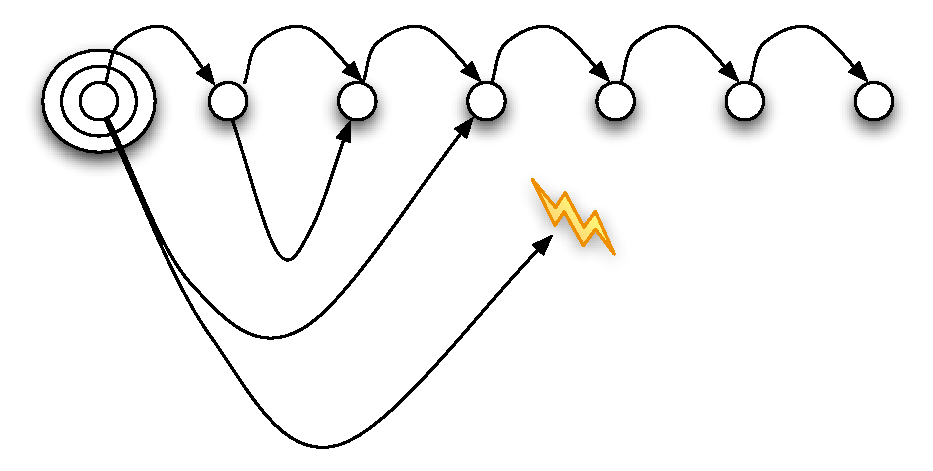
\includegraphics[width=0.75\linewidth]{figures/dedalus-time.pdf}
%   \label{fig:time}
%   %%\caption{Time moves forward in three ways: across strata, to the next fixpoint, and to some future fixpoint.}
%    \caption{Dedalus admits inferences whose consequences are visible immediately, in the next timestep, or at some unspecified timestep.}
%    
% \vspace{-8pt}
% \end{figure}

Until now we have restricted our discussion to \slang.  In this section we
introduce \lang, a superset of \slang that also admits aggregate functions
and the \emph{choice} construct.  These constructs will allow us to
express programs that establish or enforce an ordering over inputs, and to
reason about the inherent nondeterminism in communication over unreliable
networks that may delay, lose or reorder the results of logical deductions. 
%(see Figure~\ref{fig:time}).

%%\subsection{{\bf \large \lang}: New Constructs}

\subsection{Choice}

%%In this section we present the Datalog extensions missing from \slang that we will need in \lang to capture important properties of practical distributed systems.  These include aggregate functions to 
%%capture ordering constraints, and---more importantly---the choice construct to capture nondeterminacy.


%%\subsubsection{Choice}
An important property of distributed systems is that individual computers cannot control or observe the temporal interleaving of their computations with other computers.  One aspect of this uncertainty is captured in network delays: the arrival ``time'' of messages cannot be directly controlled by either sender or receiver.  In this section, we enhance our language with a traditional model of nondeterminism from the literature to capture these issues: the \emph{choice} construct as defined by Greco and Zaniolo~\cite{greedychoice}.

The subgoal \dedalus{choose((\emph{$X_1$}), (\emph($X_2$))} may appear in the body of a rule, where
\emph{$X_1$} and \emph{$X_2$} are vectors whose constituent variables occur elsewhere in the body.  Following Greco and Zaniolo, such a subgoal
enforces the functional dependency \emph{$X_1$} $\to$ $X_2$, ``choosing'' a single assignment of values to the variables
in \emph{$X_2$} for each variable in \emph{$X_1$}.

The choice construct is nondeterministic.  In a model-theoretic interpretation of logic programming, a nondeterministic program 
must have a multiplicity of stable models---that is it must be unstratifiable.  Greco and Zaniolo define 
choice in precisely this fashion: the choice construct is expanded into an unstratifiable strongly connected component of rules, 
and each possible choice is associated with a different model.

\paa{significantly, for any choice, the resulting program has a unique minimal model if the program (independent of the choice expansion)
is stratifiable, locally stratifiable, etc}  \jmh{You do need to resolve the previous paragraph, or rewrite it to simply say ``see the Italians if you want to understand more, but for our purposes assume a unique non-deterministic assignment that respects the FDs.  This allows us to have agreed-upon minimal models.''}

\subsection{Distribution Model}

A principal motivation for \lang is to model and implement distributed
systems.  To represent a distributed system, we consider some number
of agents; each running a {\em subprogram} against some subset ({\em
  horizontal partition}) of each relation's contents.  We add a column
to the beginning of each relation, then store the name of the
partition that contains each tuple in that column.  For clarity, we
say such columns are {\em location specifiers}, and prefix their
contents and the attributes that bind them with a \dedalus{\#} symbol.

Finally, we constrain \lang rules so that each rule's body contains
predicates from exactly one partition.  The head of asynchronous rules
may deduce values to be stored in any partition; an asynchronous rule
that crosses partitions in this way is called a {\em communication
  rule}.  All other rules are ``local,'' and deduce facts that are
stored in the same partition as the antecedents.

This restricts communication between nodes in two important ways.
First, by restricting bodies to a single agent, it forces all
communication between agents to occur via communication rules.  Second,
because all communication rules are asynchronous, agents may only
learn about time values at another agent by receiving messages (with
unknown delay) from that agent.  Note that this model says nothing
about the relationship between the agents' clocks; they could be
non-monotonically increasing, or they could respect a global order.
We now turn to a discussion of such issues.

\subsection{Asynchronous Rules}

In order to represent the nondeterminism introduced by distribution, we admit a
third type of rule, called an {\em asynchronous} rule.  A rule is asynchronous
if the 
%Recall our use of the distinguished variables $\Tau$ and $S$ to represent the
%time suffixes respectively in the body and head of a rule
%(Section~\ref{sec:syntaxrestrictions}).  in our discussion of \slang,
%representing the time suffixes occuring respectively in the body and head of a
%rule.
relation between the head time suffix $\SDedalus$ and the body time suffix $\Tau$ is
unknown.  Furthermore, $\SDedalus$ (but not $\Tau$) may take on the special value
$\top$ which means ``never.''  Derivation at $\top$ indicates that the
deduction is ``lost,'' as time suffixes in rule bodies do not range over
$\top$.

We model network nondeterminism using the choice construct to choose
from a value in the special 
%%\dedalus{successors} 
\dedalus{time}
predicate, which is defined using the following Datalog rules:

\begin{Dedalus}
time(\(\top\));
time(\(\SDedalus\)) \(\leftarrow\) successor(\(\SDedalus\), _);
\end{Dedalus}

\noindent
Each asynchronous rule with head predicate \dedalus{p($A_1, \ldots, A_n$)} has the following additional subgoals in its
body:

\dedalus{time($\SDedalus$), choose(($A_1, \ldots, A_n, \Tau$), ($\SDedalus$))}, 

where
$\SDedalus$ is the timestamp of the rule head.  Note that our use of \dedalus{choose} incorporates all variables of each head predicate tuple, which allows a unique choice of $\SDedalus$ for each head tuple.


\begin{example}
A well-formed asynchronous \lang rule:

\begin{Dedalus}
r(A, B, \(\SDedalus\)) \(\leftarrow\) 
  e(A, B, \(\Tau\)),
  time(\(\SDedalus\)), choose((A, B, \(\Tau\))), (\(\SDedalus\)));
\end{Dedalus}
\end{example}

We admit a new temporal head annotation to sugar the rule above.  The
identifier \dedalus{async} implies the rule is asynchronous, and stands in for
the additional body predicates.
%%$N$ is a variable,
%%corresponding to the time suffix $\Tau$ of all predicates in the rule body and
%%optionally referenced in the head.  
The above example expressed using \dedalus{async} is:

% asynchronous
\begin{example}
	A sugared asynchronous \lang rule:
	
\begin{Dedalus}
r(A, B)@async \(\leftarrow\) e(A, B);
\end{Dedalus}
\end{example}

\jmh{What do we need here?  We need to resurrect safety and strat for \lang, not just for \slang.  Monotonic deductive reductions are always cool.  Non-monotonic ones need us to ``inject'' monotonicity via the time suffix.  We lost this with async (which is natural in distributed systems).  We regain it via the addition of rules to enforce monotonicity -- these are akin to Lamport clocks and have the nice property that they don't ``cheat'', they follow our rules on messaging and asynchrony.}\rcs{tried to address this w/ following rewrite...}

Nothing in our definition of asynchronous rules prevents tuples in the
head of a rule from having a timestamp $\SDedalus$ that is less than
$\Tau$, the timestamp in the rule's antecedents. This is a significant
departure from \slang, since it violates the monotonicity assumptions
upon which we based our proof of temporal stratification.  On an
intuitive level, it may also trouble us that rules can derive head
tuples that exist ``before'' the body tuples on which they are
grounded; this violates intuitive notions of ``causality'' and admits
the possibility of temporal paradoxes.

We see no reason to restrict \lang in order to rule out such issues,
as doing so would simply reduce its expressiveness.  Recall, however,
that Algorithm~\ref{algorithm} assumed some sort of temporal
monotonicity property, which we will now define.

%
%and that with monotonicity of time, we get
%\rcs{foo}, monotonicity of rules we get \rcs{bar}, and with
%monotonicity of neither, we get unstratifiable Datalog
%programs. \rcs{everything after recall is up in the air...}

If we assume that our executions obey some causal ordering, then we
know there is some partial order over the rule derivations of the
system, and therefore, there exists at least one total ordering of the
execution that corresponds to the partial order.  Therefore, each
execution of a \lang program (which may be nondeterministic due to
\dedalus{@async}) is equivalent to the execution of some deterministic \slang
program; causality constraints reintroduce the temporal stratifiability
that our definition of \lang gave up.

Similarly, if we disallow negation, but allow derivations to pass
backwards in time, the resulting \lang program is still temporally
stratifiable.  However, admitting both negation across timesteps and
causality violations leads to an underlying Datalog program that is
unstratifiable.

We note that non-causal schedulings are of practical importance;
distributed systems built atop unreliable and asynchronous primitives
could very well observe seemingly nonsensical orderings.  For example,
in scalable internet publishing application, one can imagine that, due
to caching or failure, it is possible that comments begin to arrive
over the network well before the article they respond to.

\subsubsection{Entanglement}

Consider the asynchronous rule below:

\begin{Dedalus}
p(A, B, N)@async \(\leftarrow\)
  q(A, B)@N;
\end{Dedalus}

Due to the async keyword in the rule head, each \emph{p} tuple will take some unspecified time suffix value.
Note however that the time suffix $N$ of the rule body appears also in an attribute of \emph{p} other than the time suffix, recording a 
binding of both the time value of the deduction and the time value of its consequence.  We call such a binding
an \emph{entanglement}.   Entanglement is a surprisingly powerful construct that allows a rule to 
reference the logical clock time of the deduction that produced one (or more) of its subgoals.  Note that in order
to write the rule it was necessary to not sugar away the time suffix in the rule body.  We restrict the use of entanglements to asynchronous rules. \jmh{Why the restriction?  Also, can you justify that it's surprisingly powerful?}

\jmh{Where do we give the def that say ``\lang is \slang with the following extra goo''?  Here?  After async?}\rcs{beginning of sec 6, first sentence}

\subsection{Lamport Clocks}

Recall that \lang allows program executions to violate causality.
This section explains how to implement Lamport
clocks~\cite{timeclocks} atop \lang, which allows programs to ensure
temporal monotonicity\rcs{term}, by reestablishing a causal order,
despite derivations that may flow backwards through time.

Consider a rule \dedalus{p(A,B)@async \(\leftarrow\) q(A,B)}.  By
rewriting it to:

\begin{Dedalus}
persist[p, 2]
p\_wait(A, B, N)@async \(\leftarrow\) q(A, B)@N;
p\_wait(A, B, N)@next \(\leftarrow\) p\_wait(A, B, N)@M, N \(\ge\) M;
p(A, B)@next \(\leftarrow\) p\_wait(A, B, N)@M, N < M;
\end{Dedalus}

we place the derived tuple in a new relation \dedalus{p\_wait} that
stores any tuples that were ``sent into the past'' until the point in
time at which they were derived.  Conceptually, this causes the system
to evaluate a potentially large number of timesteps (if N is
significantly less than the timestamp of the system when the tuple
arrives).  However, if the runtime is able to efficiently evaluate
timesteps when the database is quiescent (by recognizing that the
timesteps can be skipped, as is done in Algorithm~\ref{alg:tsn}), then
instead of ``waiting'' by evaluating timesteps, it will simply
increase its logical clock to match that of the sender.  In contrast,
if the tuple is ``sent into the future,'' then it is processed using
the timestep that receives it.

This manipulation of timesteps and clock values is equivalent to
conventional descriptions of Lamport clocks, except that our Lamport
clock implementation also needs to events in order to avoid causality
violations.  Therefore, it needs to temporarily store incoming tuples
in the \dedalus{p\_wait} relation.

Note that we gloss over one detail here; Lamport clocks rely
upon a ``tie-breaking'' function to ensure that no two events have the
same timestamp.  In practice, such a function could be implemented by
appending a unique node identifier to each timestamp; this could be
done automatically by the runtime, or by adding arithmetic expressions
or other computations to the rewritten predicates.

\jmh{Can't we please do the normal use of Lamport clocks, i.e. show how it solves a distributed systems problem?}
\rcs{I'd like to do this, but don't have any good examples...}
